\subsection{Progettazione di dettaglio e codifica}
Periodo: dal \textbf{2022-02-20} al \textbf{2022-03-13} \mbox{} \\ \mbox{} \\
Le precondizioni sono:
\begin{itemize}
	\item le postcondizioni della fase precedente sono state soddisfatte.
\end{itemize} \mbox{} \\
Le postcondizioni sono:
\begin{itemize}
	\item aggiornamento e approvazione dei documenti prodotti precedentemente;
	\item completamento codifica e verifica;
	\item realizzazione dei diagrammi delle classi e dei diagrammi delle attività;
	\item redazione del manuale utente;
	\item realizzazione della presentazione da esporre nella seconda revisione: la \textit{Product Baseline}\glo{}. 
\end{itemize} \mbox{} \\
La fase è composta da dieci incrementi e quattro nuove attività:
\begin{itemize}
	\item \textbf{Incremento e verifica dei documenti}: viene aggiornata e migliorata la documentazione;
	\item \textbf{Incremento e verifica delle attività}: viene migliorata l’attività di \textit{Technology Baseline}\glo{}, incrementando lo studio delle tecnologie e progettando ad alto livello come realizzare il prodotto finale;
	\item \textbf{Specifica tecnica}: viene realizzato un documento contenete tutte le caratteristiche del prodotto e le motivazioni che hanno portato alla loro scelta;
	\item \textbf{Product Baseline}: segue la \textit{Technology Baseline}, la quale si compone di 3 incrementi:
		\begin{itemize}
			\item \textbf{Design Pattern\glo{}}: vengono approfonditi con lo scopo di capire quali usare nel progetto;
			\item \textbf{Diagrammi delle Classi}: vengono realizzati i diagrammi delle classi;
			\item \textbf{Diagrammi delle Attività}: vengono realizzati i diagrammi delle attività.
		\end{itemize}
	\item \textbf{Codifica}: dopo aver realizzato il PoC nella fase precedente, si procede alla scrittura del codice. L'attività di codifica si divide in due incrementi ciclici consecutivi con relativa verifica e ciascun incremento è costituito dalla codifica di alcuni casi d'uso\glo{}, sulla base di quanto precedentemente progettato. L’associazione di un determinato numero di casi d’uso in ogni incremento ha lo scopo di concludere l'attività di codifica con l’implementazione di tutti gli UC obbligatori, come indicato nell'\textit{Analisi dei Requisiti}. \\ Se alla fine di un incremento si osservasse il mancato completamento di quanto prestabilito, quest’ultimo verrà accorpato al successivo o verrà ripianificata l’attività di codifica per quel periodo. Se l'attività di codifica si dovesse concludere prima del previsto, il tempo avanzato dovrà essere impiegato per realizzare i casi d'uso opzionali. I due incrementi sono così programmati:
		\begin{enumerate}
			\item \textbf{Incremento 1}: nel primo incremento l'attenzione del gruppo sarà focalizzata sulla realizzazione dei casi d'uso più importanti, ovvero di UCW7, UCW8, UCW9, UCW10, UCW11, UCW12 e UCW13;
			\item \textbf{Incremento 2}: nel secondo incremento il gruppo si focalizza sull'implementazione dei casi d'uso d'errore, di quelli relativi alla registrazione dell'utente e all'area personale, ossia UCW1, UCW2, UCW3, UCW4, UCW5 e UCW6.  
		\end{enumerate}
	\item \textbf{Manuale Utente}: viene redatto un documento specifico per l'utente con le istruzioni d'uso, il quale ha lo scopo di aiutare e agevolare l’utente nell’uso del prodotto da noi fornito.
\end{itemize}

\subsubsection{Periodi}

Questa fase viene a sua volta suddivisa in quattro periodi, scanditi da milestones pianificate all'interno del gruppo:

\subsubsubsection{I Periodo}
\textbf{dal 2022-02-20 al 2022-02-22:} In questo primo periodo il gruppo si dedicherà a migliorare i documenti e affinare le tecnologie per iniziare la codifica.

\subsubsubsection{II Periodo}
\textbf{dal 2022-02-22 al 2022-03-01:} Nel secondo periodo, il gruppo dovrà aver compreso e ultimato la \textit{Product Baseline} con i relativi diagrammi e design pattern.

\subsubsubsection{III Periodo}
\textbf{dal 2022-03-01 al 2022-03-08:} Nel terzo periodo il team si focalizzerà sulla codifica del primo incremento. Inoltre, dovranno essere iniziate sia la stesura relativa alla specifica tecnica che il manuale utente.

\subsubsubsection{IV Periodo}
\textbf{dal 2022-03-08 al 2022-03-13:} Nell'ultimo periodo il gruppo ultimerà la codifica con l’ultimo incremento e terminerà i documenti di specifica tecnica e manuale utente.

\begin{figure}[H]
\centering
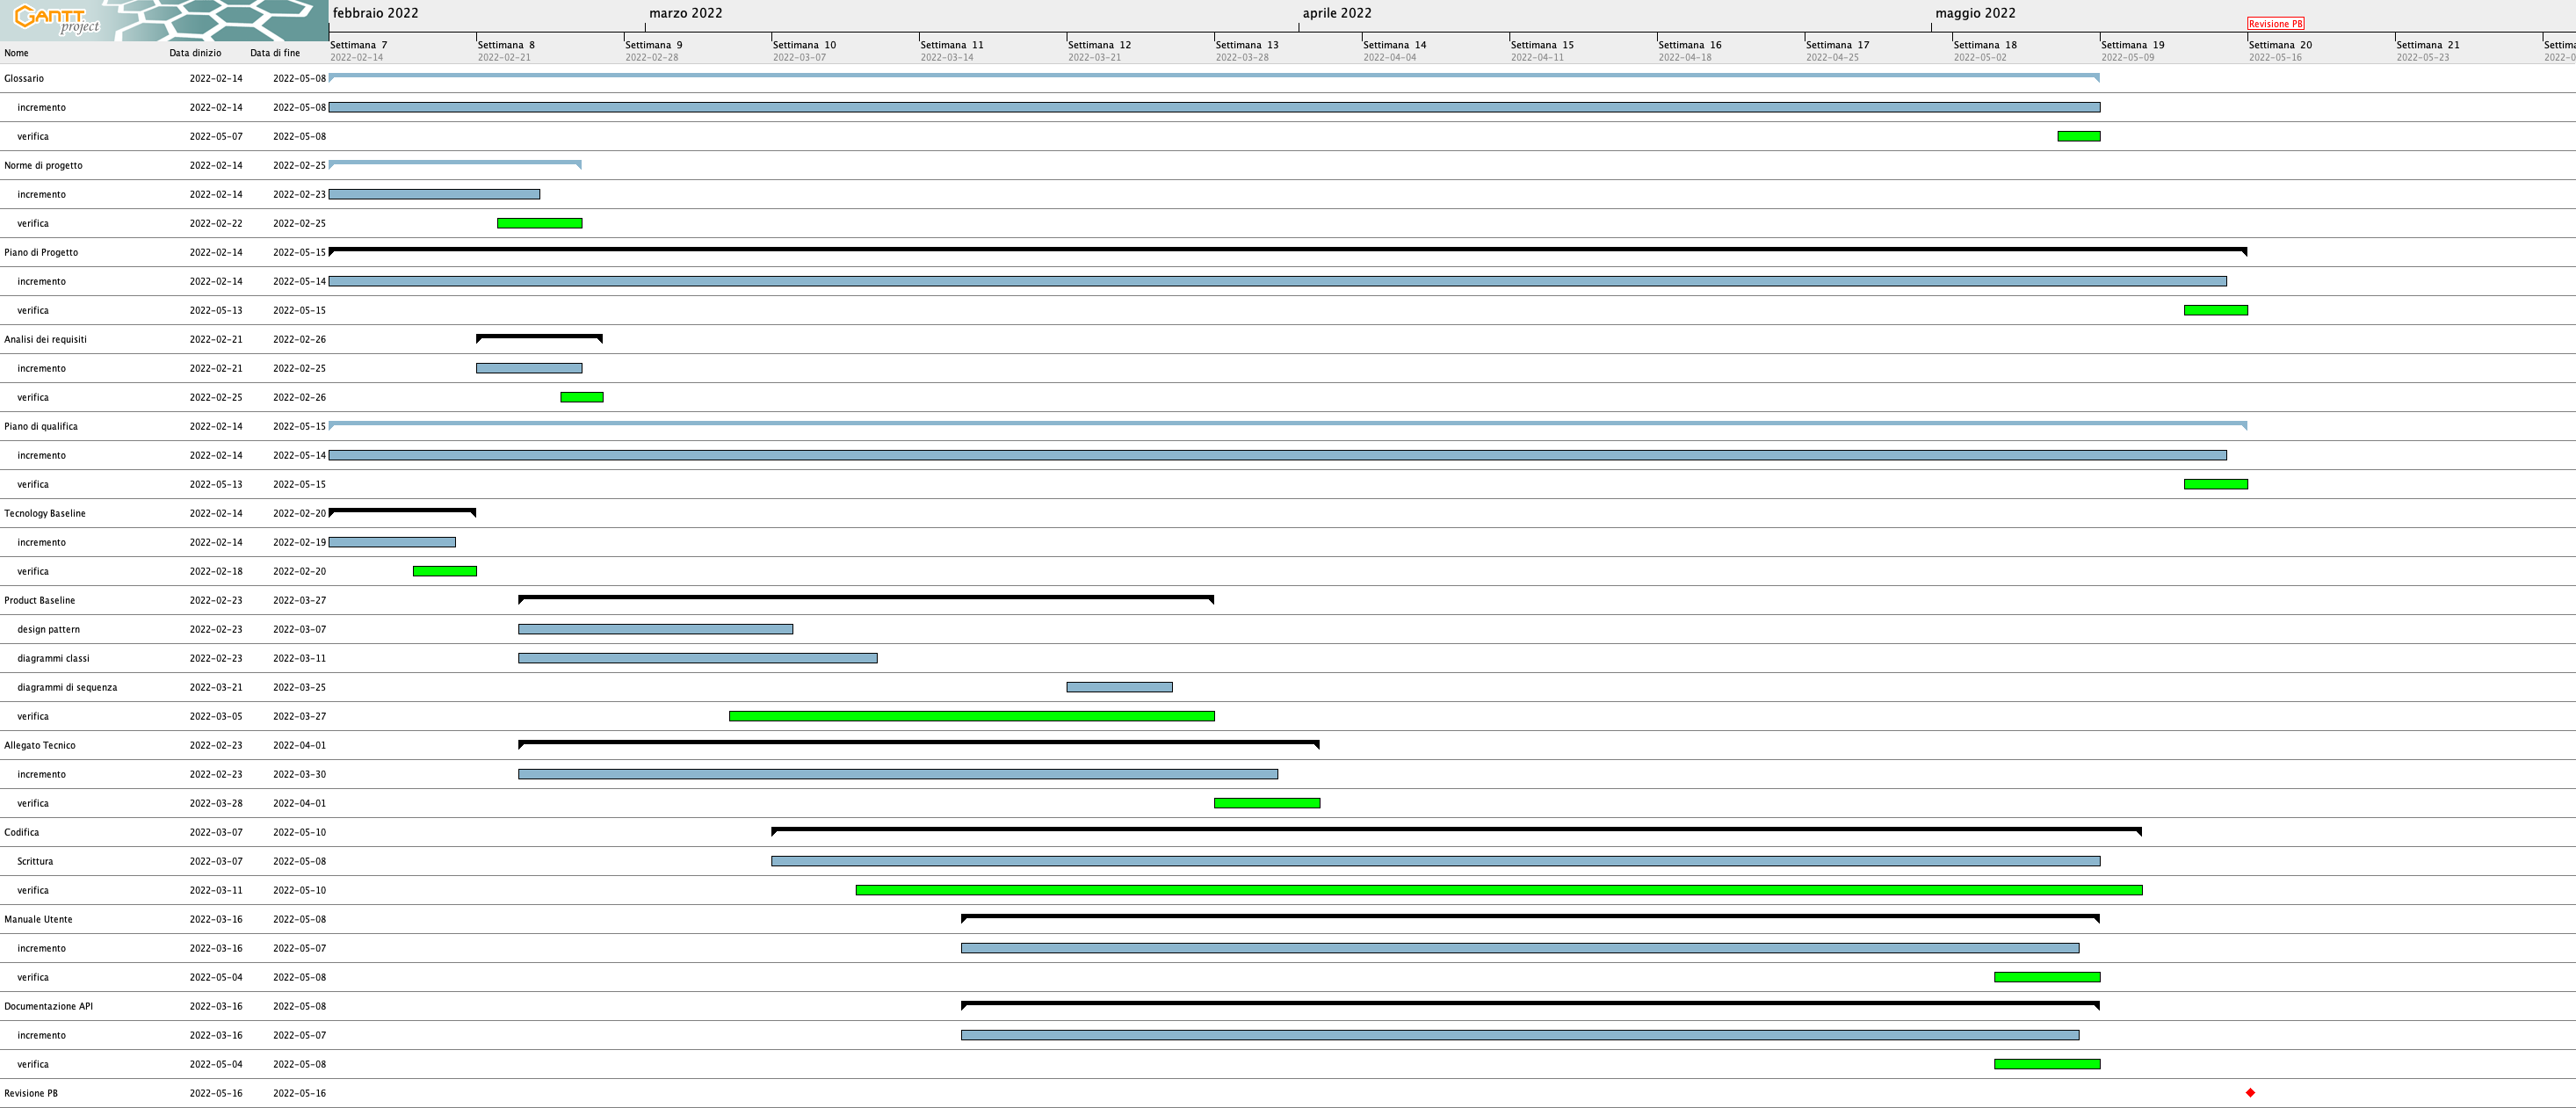
\includegraphics[scale=0.35]{Sezioni/gantt/progettazione_codifica.png}
\caption{Diagramma di Gantt - Progettazione e codifica}
\end{figure}